\section{Chapter 2: Radar system overview}

In this chapter we introduce a few fundamental radar concepts which will be important for understanding the data acquired by the 60 GHz sensor.
\\ \\
The radar equation.
\\ \\
The matched filter.
\\ \\
The IQ demodulation scheme. 
\\ \\
The radar system used for this project is a 60 GHz radar developed by Acconeer AB.



\subsection{The radar principle}

The radar principle is at its core simple.  A wavelet pulse $x_T(t)$ with some carrier frequency $\Omega$  is transmitted towards an object of interest. After some short time $t_1$, the radar listens for an echo. If no echo is received, it means there is no object present at distance\footnote{The reason for dividing by 2 is that the wavelet pulse must first travel from the radar to the object, and then find its way back to the radar.}
\begin{equation}
	d_1 = \frac{v_0\cdot t_1}2
\end{equation}
where $v_0$ is the speed of an electromagnetic wave in air. After the previously transmitted wavelet is guaranteed to have died out, a new one is transmitted. Again, the radar listens for an echo, but this time after another time $t_2$ has passed. $t_2$ is greater than $t_1$, meaning the radar listens for echoes further away. If an echo is received, it means there is an object present at distance 
$
	d_2 = \frac12(v_0\cdot t_2).
$
This process is repeated for different time delays $t_i$. The chosen time delays can be adjusted depending on in what ranges one wants to search in, and how good range resolution one seeks.

Together, the echoes (or lack thereof) from each transmitted wavelet make up one sweep. A sweep is often plotted in an amplitude-vs-range, or amplitude-vs-depth diagram as in figure (...). This plot is a good way to visualize at what ranges objects are present.

* Plot of sweep *

\subsection{Elements of a pulsed radar}

A pulsed radar system can be realized in countless ways, but all subscribe to the fundamental physical laws of electromagnetic radiation previously described. In this section one such configuration for a pulsed radar system is described.

A waveform generator outputs a radar envelope which is modulated by a local oscillator to some desired radio frequency. After signal amplification the wavelet is transmitted through an antenna. 

Detection is performed by a second antenna, which receives the returning signal during some time interval. The received signal then goes through a process known as \emph{mixing}. An internal wavelet is generated at a very specific delay from the initial pulse transmission and multiplied with the received signal. If the received and internal pulses do not match, the output of this multiplication will be zero. If there however exist some overlap between the internal and returning signals the output will be nonzero, indicating some level of energy content at the distance corresponding to the internal pulse delay. By increasing the internal pulse delay and repeating this procedure a set of measurement points is obtained. Mixing is thus achieved by multiplying a large number of returning wavelets with internally generated wavelet counterparts, adding a slight delay between sampling points. 


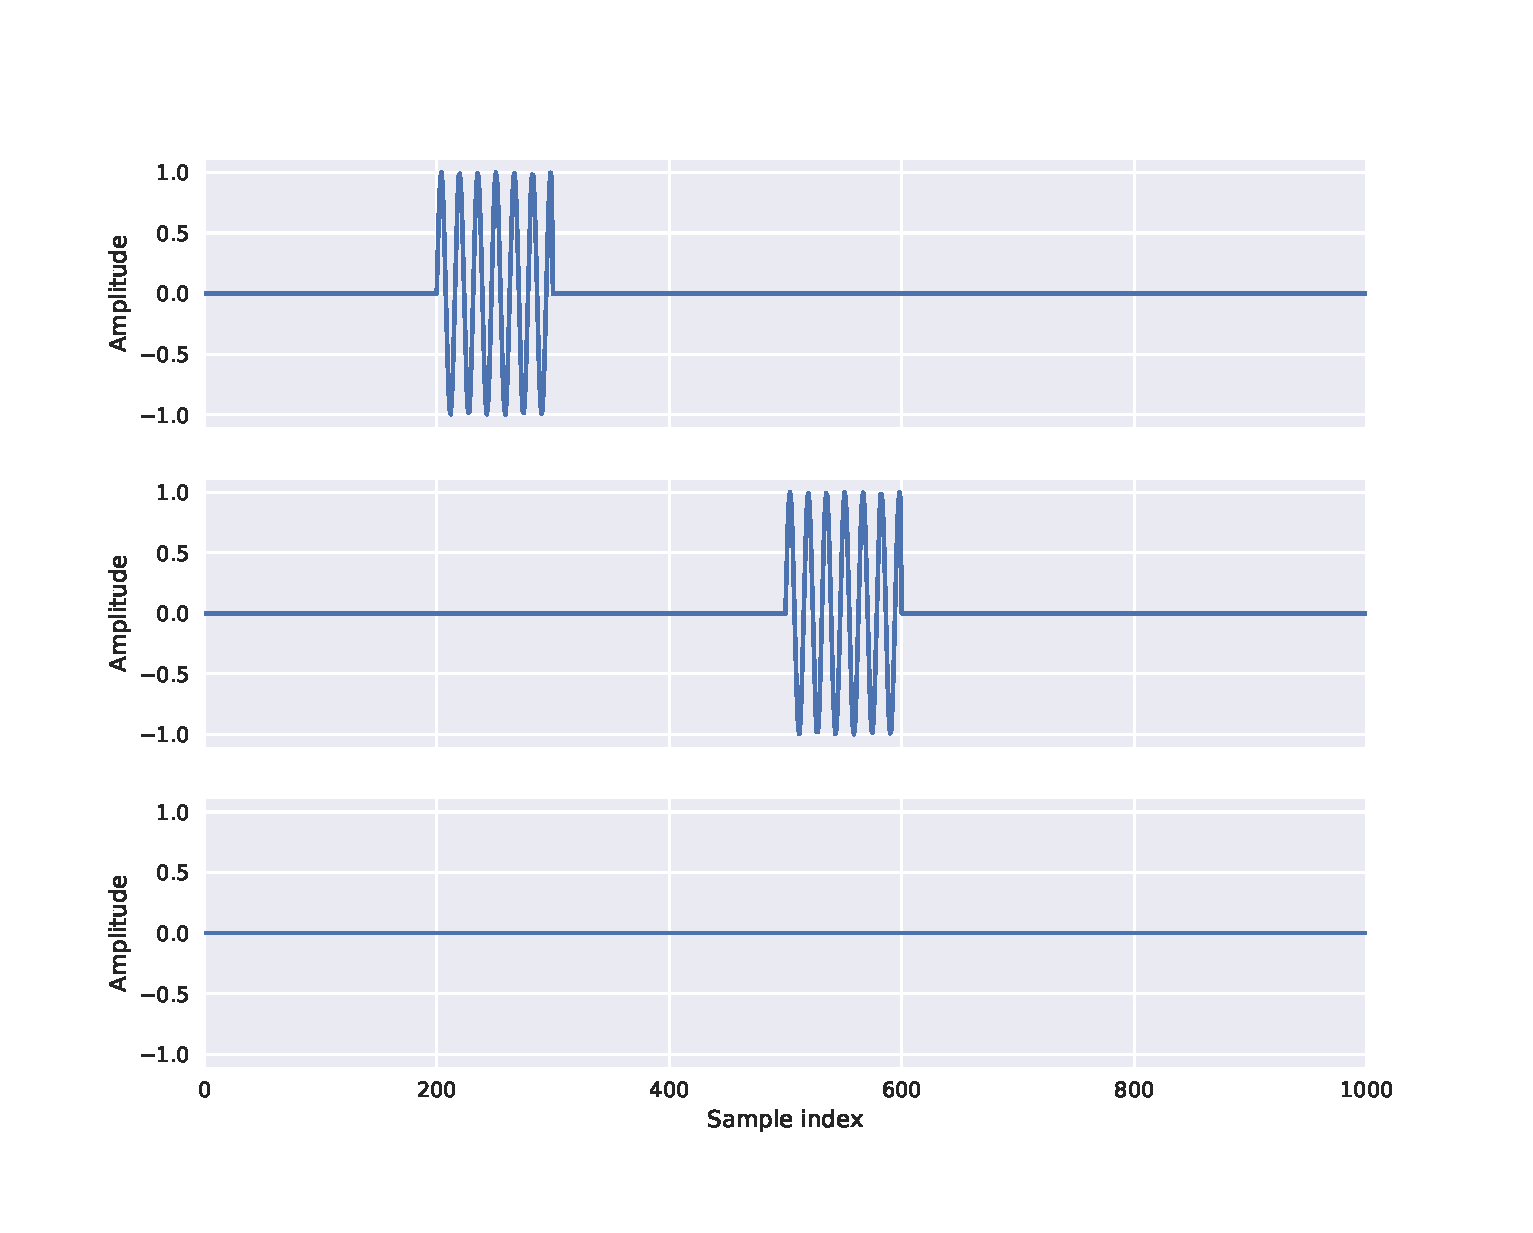
\includegraphics[scale=0.5]{figs_temp/mixing0}

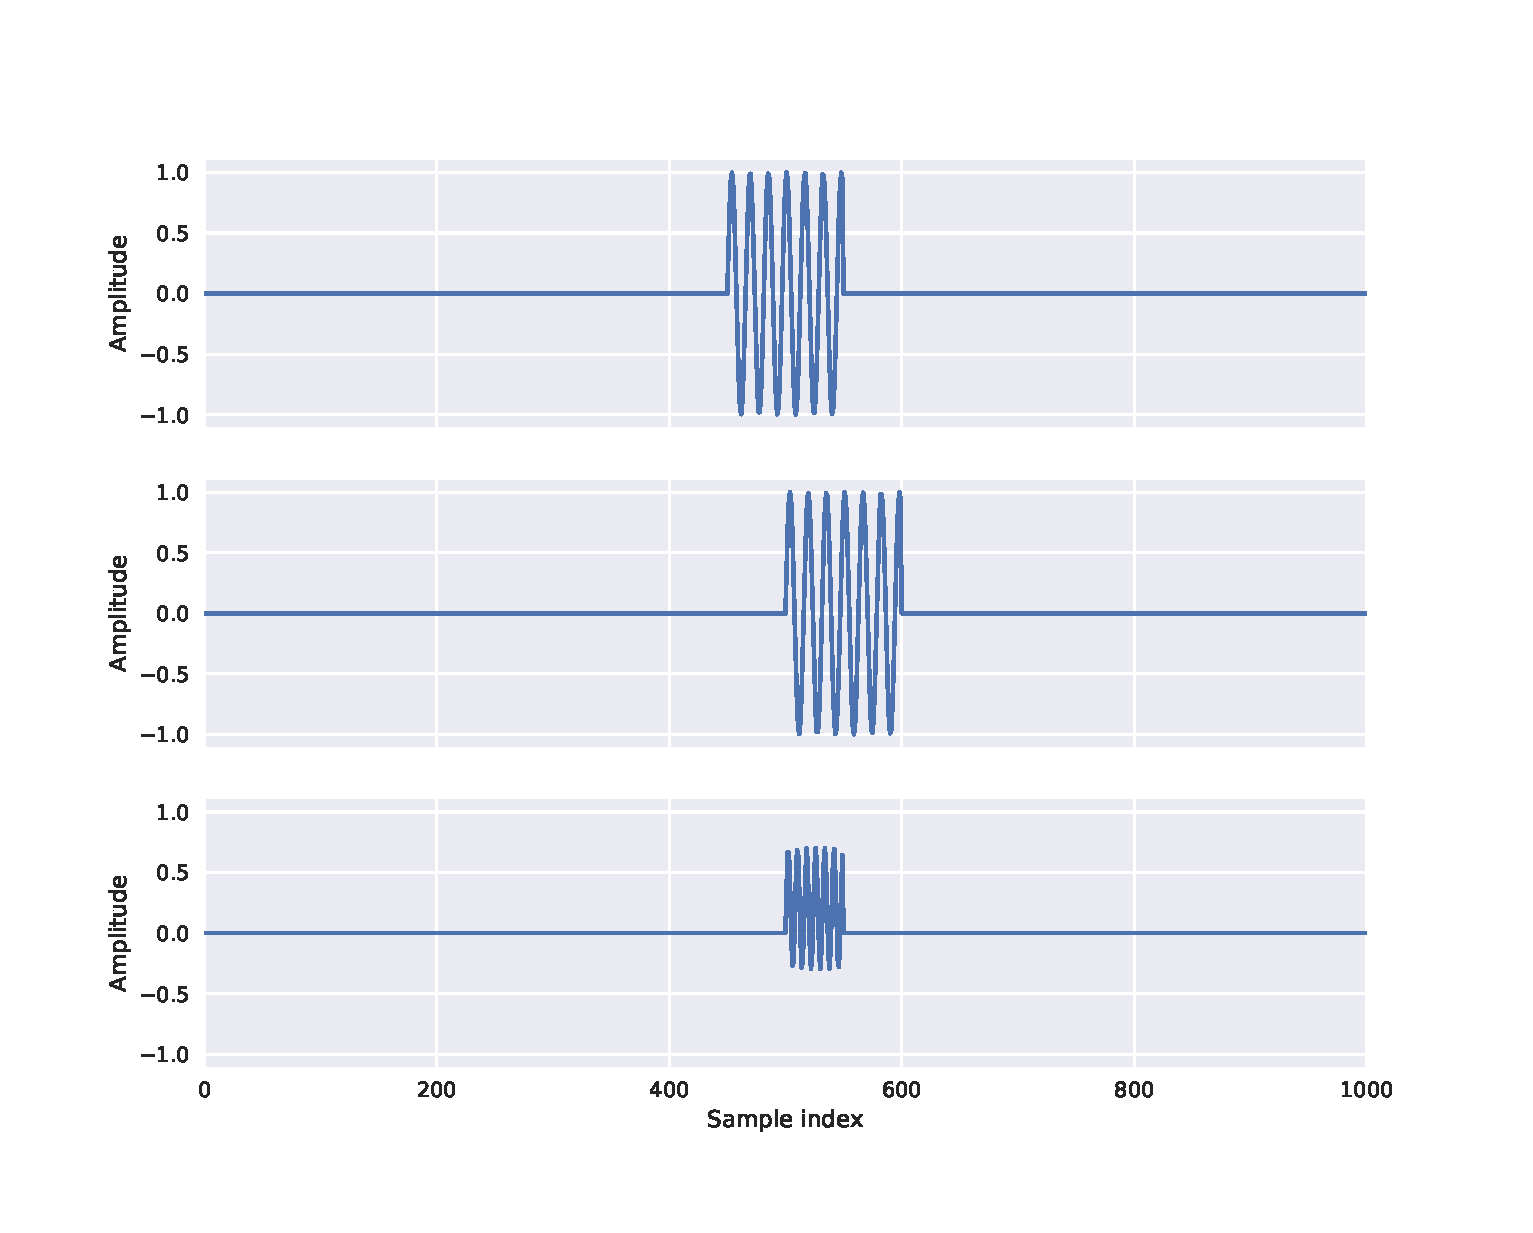
\includegraphics[scale=0.5]{figs_temp/mixing1}

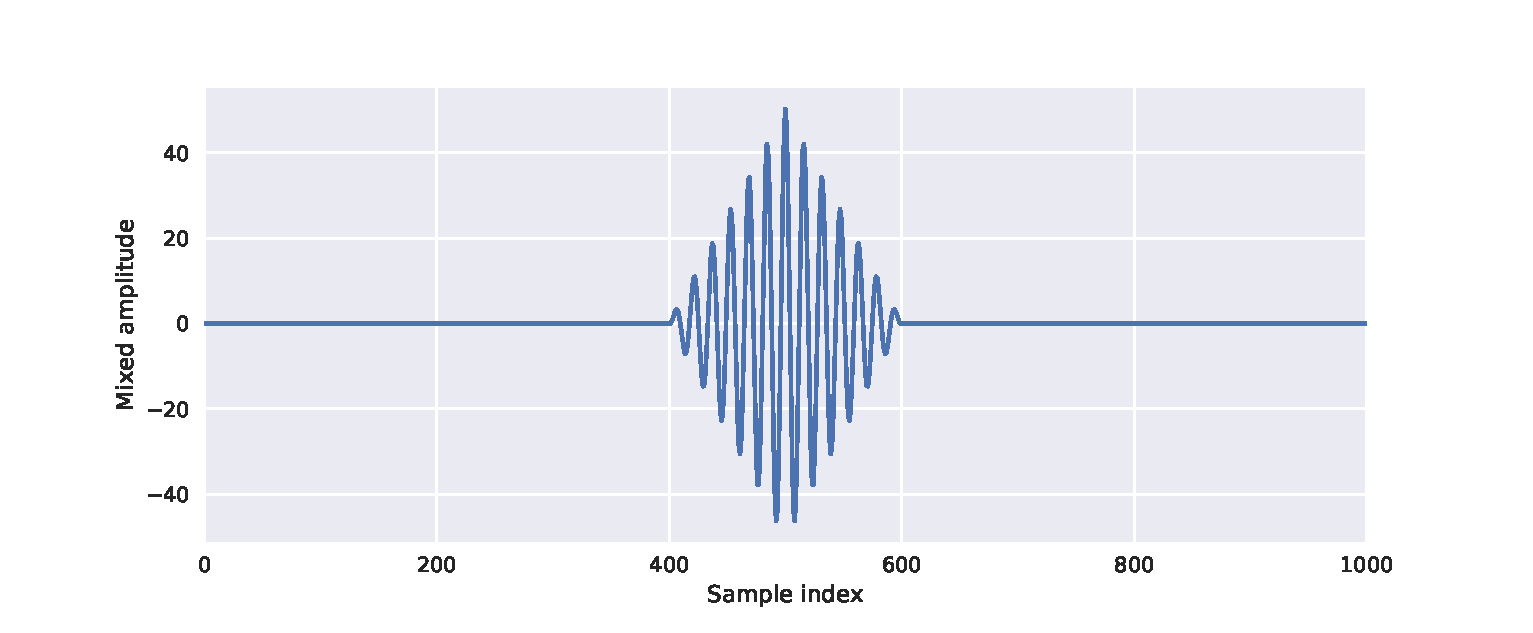
\includegraphics[scale=0.5]{figs_temp/mixing2}




\subsection{IQ Data}
A common type of data when working with radar signal processing is in-phase and quadrature-phase data (IQ-data).  This type of data is useful in that it contains information not only about amplitude, but about the phase of the radar signal as well \citep{richards_2014}. IQ-data is represented as complex numbers, and a radar sweep consists of several such complex numbers - one for each investigated range. To obtain the amplitude plot, as the one in figure .... for a sweep, $s$, made up of IQ-data, one simply computes the absolute value for each complex number in $s$. Similarly, a phase curve can be obtained by computing the phase in each point. A phase curve can typically look like the one in *Figure of phase plot*

In many applications, the phase information in IQ-data is used when small changes in the radar signal need to be detected, (Mention a case such as recording over grass...) as the phase is more sensitive to changes than the amplitude \citep{lien_gillian_karagozler_amihood_schwesig_olson_raja_poupyrev_2016}. If an object is detected at distance $r(t_1)$ from the radar at time $t_1$, and shortly thereafter, the object is moved to distance $r(t_2)$, the corresponding difference in phase will be
\begin{equation}
	\label{eq:phase_diff}
	\Delta\phi(t_1, t_2)=\frac{4\pi}{\lambda}(r(t_2)-r(t_1)) \quad\quad \textrm{mod 2$\pi$}
\end{equation}
By having a sampling frequency which is too low, the range difference in $\eqref{eq:phase_diff}$ could potentially become very big, and the phase difference would fluctuate over time and be incomprehensible.

In the case of material classification, a high sampling frequency is highly beneficial. When moving across surfaces characterized by tiny details, a high sampling frequency is essential in capturing the shape of these.

For a thorough description of how IQ-data is derived from raw radar data, we refer to \citep{richards_2014}

\section{Data}
\subsection{Data Collecting}
Having reliable data is a fundamental requirement in building a good model. There are many parameters to consider in optimizing the data collecting process. However,  finding an optimal solution is often impossible as the combinations are endless, but putting some thought into every decision often proves worthwhile. Below, we motivate our choices of sensor placement as well as various parameters.

\subsubsection{Measurement Setup}


Include graphics of the sensor placement etc. and describe the setup briefly. Possibly mention the $\frac14\lambda$ gap between the sensor and RLM plastic.
\subsubsection{Measurement Settings}
Having reliable data is a fundamental requirement in building a good model. Hence, choosing suitable parameters such as sampling frequency, regions of interest and planning a good measurment setup are all crucial tasks. The sampling frequency is particularly important to consider when working with means that could potentially cause aliasing. One such case is the DFT \citep{lindgren_rootzeŽn_sandsten_2013}. If the sampling frequency is too low, we get aliasing etc. etc. 

In order to assure that aliasing is avoided, the maximal frequency component registered by the radar must be surpassed by half the sampling frequency
\begin{equation}
	f_{max} < \frac{f_s}{2}.
\end{equation}
The sampling frequency can be chosen accordingly, assuming the maximal frequency component is known. 

In figure (fig. from previous subsubsection) a vehicle is moving forward with constant speed, having a sensor mounted at the front. As it moves forward, small objects on the ground get closer to the radar sensor with some speed. This gives rise to a doppler frequency being registered by the radar, which is \citep{lien_gillian_karagozler_amihood_schwesig_olson_raja_poupyrev_2016}
\begin{equation}
	f_{d} = \frac{2v_\perp}{\lambda}.
\end{equation}
...


\subsection{Chapter 2.5: Data exploration}

Good source on PCA
\cite{hyvasrinen_karhunen_oja_2004}
PCA 125-143

Information theory
105-122
Argument for downsampling in range: In an information theoretic framework we interpret a random variable by how unpredicable or unstructured an observation of the variable is. This concept, examining the randomness of a variable, is commonly measured through entropy. Directly related to entropy is mutual information which essentially is how much information each member of a set have on the other members. \cite{hyvasrinen_karhunen_oja_2004}. Ideally one wants measurements that have a low measure of mutual information, meaning that each datapoint contain information not found elsewhere in the set. 

Observing a typical radar sweep[ref to plot with sweep] we note that points are very closely related on a small range scale, and nearly identical if we were to examine them on a sample by sample basis. One could argue that the mutual information found in the set is very high and that the entropy in each datapoint is low. Hence, to lower the first and increase the latter, one could downsample by some factor $D$ in range without significant loss of information.


PCA 125-143: Through the point and feature selection methods described in previous sections we obtain high dimensional feature vectors. Getting an intuitive feel for such data extracted in these processes is difficult as direct plotting is limited to three dimensions. 

Principal Component Analysis (PCA) is  a classical technique in statistical data analysis which takes a large set of multivariate variables and finds a smaller set of variables with less redundancy. Critically, PCA finds a rotated orthogonal coordinate system such that the elements of the set become uncorrelated. Projecting elements on the principal axes corresponding to the directions of maximal variance a good approximation of the original data in lower dimension is obtained \citep{hyvasrinen_karhunen_oja_2004}. 
